\sect{Kellerautomaten}

Ein \textbf{Kellerautomat} ist ein EA für die Erkennung von kontextfreien Sprachen mit unbegrenztem Stack (Keller, Stapel).

\textbf{Kelleroperationen:}

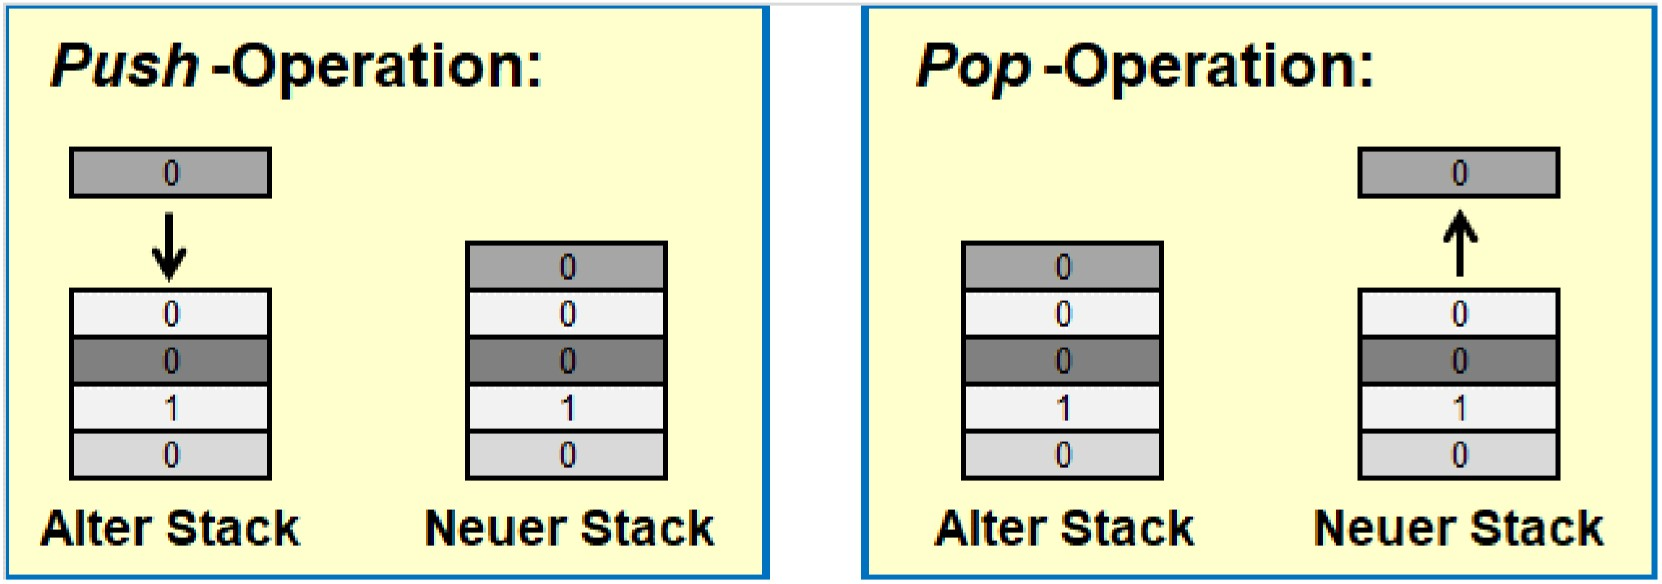
\includegraphics[scale=0.155]{kelleroperationen}

Ein \textbf{deterministischer Kellerautomat} $M$ ist ein 7-Tupel $(Q, \Sigma, \Gamma, \delta, q_0, \$, F)$ mit
\begin{itemize}
    \item $Q$ ist die endliche Menge von Zustände
    \item $\Sigma$ ist das Alphabet der Eingabe
    \item $\Gamma$ ist das Alphabet des Kellers
    \item $\delta: Q \times (\Sigma \cup \varepsilon) \times \Gamma \rightarrow Q \times \Gamma^*$ ist eine (partielle) Übergangsfunktion
    \item $q_0 \in Q$ ist der Startzustand
    \item $\$ \in \Gamma$ ist ein ausgezeichnetes Symbol vom Alphabet des Kellers
    \item $F \subseteq Q$ ist die Menge der akzeptierenden Zustände
\end{itemize}
Anfangs enthält der Keller eine Instanz des Symbols $\$$.

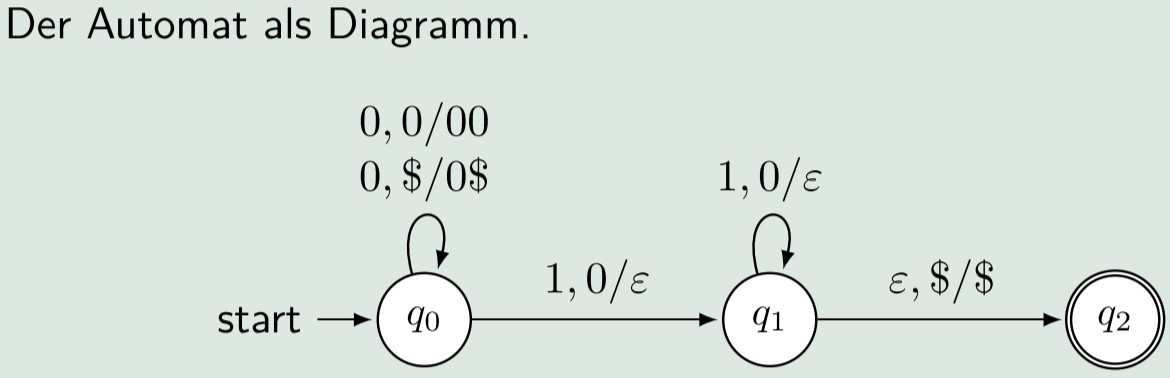
\includegraphics[scale=0.22]{kellerautomat}

Das Zeichen $\$$ steht für einen leeren Stack.

Ein \textbf{Berechnungsschritt} $\delta(q, \textcolor{Green}{b}, \textcolor{red}{c}) = (p, \textcolor{blue}{\omega})$ wird wie folgt interpretiert:
\begin{enumerate}
    \item Aktueller Zustand $q$
    \item Lese Symbol $\textcolor{Green}{b}$ von der Eingabe (falls $b = \varepsilon$ wird nichts gelesen)
    \item Entferne das oberste Kellersymbol $\textcolor{red}{c}$
    \item Schreibe Wort $\textcolor{blue}{\omega}$ auf den Stack
    \item Wechsle in den Zustand $p$
\end{enumerate}

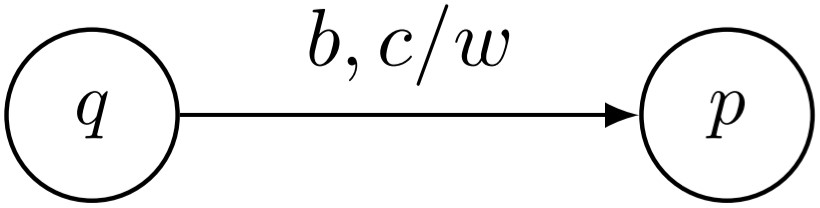
\includegraphics[scale=0.15]{uebergang-kellerautomat}

Ein \textbf{nichtdeterministischer Kellerautomat} unterscheidet sich nur in der Übergangsfunktion:\\
$\delta: Q \times (\Sigma \cup \varepsilon) \times \Gamma \rightarrow \mathcal{P}(Q \times \Gamma^*)$

\begin{itemize}
    \item Die Zusatzbedingung der Übergangsfunktion fällt weg
    \item Analog zum NEA bildet die Übergangsfunktion des NKA in die Potenzmenge ab
\end{itemize}

\textbf{Beispiel NKA:}

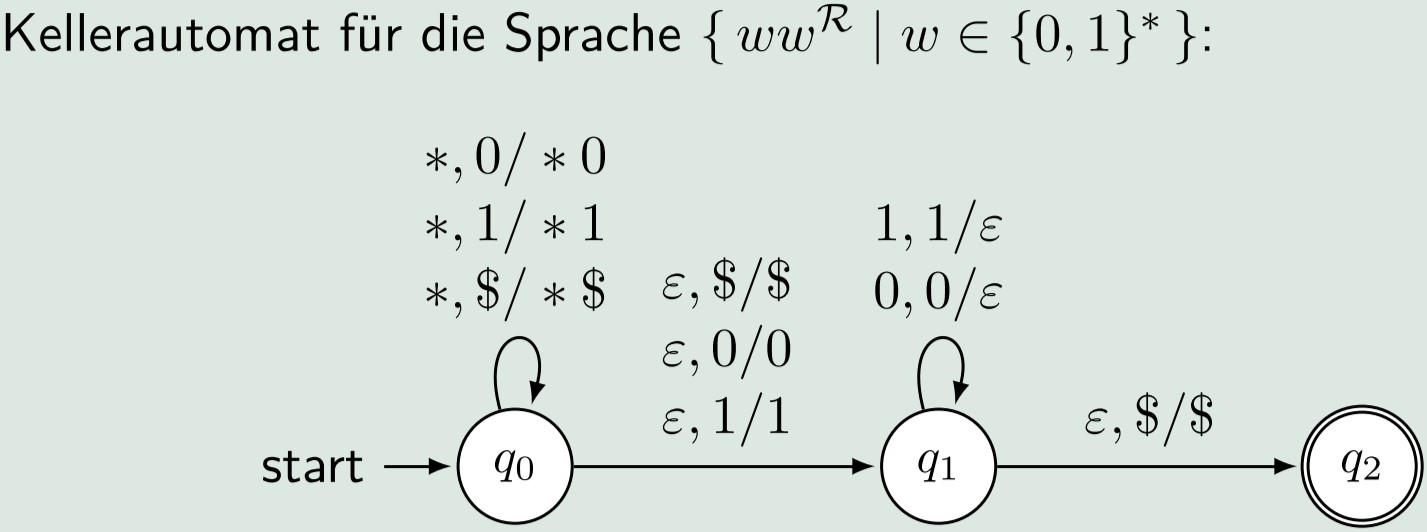
\includegraphics[scale=0.175]{kellerautomat-nka}

Der * steht für ein beliebiges Zeichen aus $\Sigma$

\textbf{Beispiel:} Gegeben sei $M_1$ (für die Sprache $L = \{ 0^n 1^n \mid n > 0 \}$) und die Wörter $w' = 0011$ und $w'' = 011$

Die Berechnungen für $w'$ lautet:

$(q_0, 0011, \$) \vdash (q_0, 011, 0\$) \vdash (q_0, 11, 00\$) \vdash (q_1, 1, 0\$) \vdash (q_1, \varepsilon, \$) \vdash (q_2, \varepsilon, \$) \\
\Rightarrow \text{ Akzeptierend}$

Die Berechnung für $w''$ lautet:

$(q_0, 011, \$) \vdash (q_0, 11, 0\$) \vdash (q_1, 1, \$) \vdash (q_2, 1, \$)$ \\
$\Rightarrow$ Kein weiterer Schritt möglich, d.h.\ nicht akzeptierend

\textbf{Satz:} Eine Sprache ist genau dann kontextfrei, wenn es einen NKA gibt, der die Sprache erkennt.
\begin{itemize}
    \item Nicht jede kontextfreie Sprache, die von einem NKA erkannt wird, wird von einem DKA erkannt.
    \item Kontextfreie Sprachen, die von einem DKA erkannt werden, sind eindeutig.
\end{itemize}